\section{Sizing the axes}
\label{section_sizing_axes}
\subsection{External versus internal lengths and coordinates}
As mentioned above, the origin and coordinates within "axis" will in
general not be the same as the coordinates and origin within
"tikzpicture" but outside "axis".  This is inevitable if we expect
coordinates in "tikzpicture" to be based in 1 centimeter units, but
coordinates within "axis" to match the numbers displayed in the axes.
The next example illustrates this difference: 

\noindent
\begin{minipage}{0.48\columnwidth}
\begin{latex}
\begin{tikzpicture}
\begin{axis}["title={Diagonal 1cm up 
       and over}"]
\end{axis}
\draw (0,0) -- (1,1);
\end{tikzpicture}
\end{latex}
\end{minipage}
~~%
\begin{minipage}{0.48\columnwidth}
\begin{latex}
\begin{tikzpicture}
\begin{axis}[xmin = 0, xmax=1, ymin=0, ymax=1,
"title={Diagonal 1 internal unit up and over}"]
\draw (0,0) -- (1,1);
\end{axis}
\end{tikzpicture}
\end{latex}
\end{minipage}

\begin{center}
\tikzcount
\begin{minipage}{\columnwidth}
\raisebox{0.5cm}{1cm \rule{2pt}{1cm}}
\begin{tikzpicture}
\begin{axis}[title={Diagonal 1cm up and over}]
\end{axis}
\draw (0,0) -- (1,1);
\end{tikzpicture}
~~
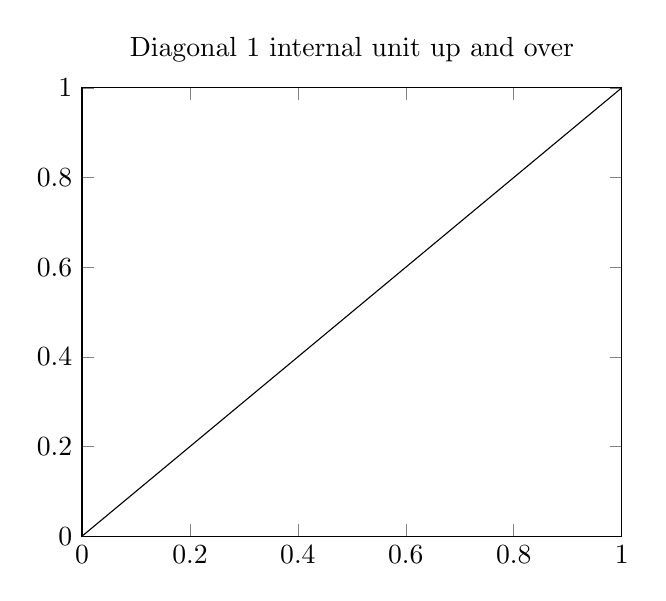
\begin{tikzpicture}
\begin{axis}[xmin = 0, xmax=1, ymin=0, ymax=1,
title={Diagonal 1 internal unit up and over}]
\draw (0,0) -- (1,1);
\end{axis}
\end{tikzpicture}\\
\hspace*{1.5cm}\rule{1cm}{2pt}\\
\hspace*{1.5cm} 1cm
\end{minipage}
\tikzcount
\end{center}
\noindent We've added two markers, created with "\rule" outside of the
"tikzpicture" so you can see what a real centimeter is. Between "axis"
and "tikzpicture" (i.e. outside "axis" but inside "tikzpicture") a
coordinate of 1 means 1cm from the origin, where 1cm is what we would
get if we printed it out and put a ruler on the result (assuming we
have not used a "scale" option, or similar change, in "tikzpicture").
But inside "axis" a coordinate of 1 uses the numbers shown in the
coordinate axes, and therefore a length of 1 is also measured using
these coordinates.  When we need to distinguish between these two ways
of measuring lengths we'll call the former, ``external'' and the
latter ``internal''.  In other words, the ``external width'' of a
figure is what we could get by measuring it with a ruler, or what TeX
will see in terms of a box on the page, the lengths marked by "\rule"s
above, and the ``internal width'' is what we would get using the
numbers on the axes.  External dimensions can be set manually directly
using the "width" and "height" keys, and internal size can be manually
directly set by using "xmin", "xmax", "ymin" and "ymax".

The figure below has an external size of approximately
240pt~$\times$~207pt (that's width~$\times$~height) and internal size
of approximately 10,000,000~$\times$~10,000,000.
\begin{latex}
\begin{tikzpicture}
\begin{axis}["tick scale binop"={\times}]
  % pgfplots knows 1e6 notation for 10^6 
  \addplot "coordinates {(1e6,1e6) (1e7,1e7)}";
\end{axis}
\end{tikzpicture}
\end{latex}
%
\begin{center}
\tikzcount
\begin{minipage}{\columnwidth}\centering
207pt = \rule[-103.5pt]{2pt}{207pt} \quad 
\raisebox{-0.5\height+2pt}{%
\color{red}\fbox{%
\color{black}
\begin{tikzpicture}
\begin{axis}[tick scale binop={\times}]
\addplot coordinates {(1e6,1e6) (1e7,1e7)};
\end{axis}
\end{tikzpicture}}}\\[10pt]
\hphantom{207pt = \rule[-103.5pt]{2pt}{207pt} \quad }\rule{240pt}{2pt}\\
=240pt
\end{minipage}
\end{center}
Note: according to the "pgfplots" manual the external dimensions are
\emph{approximately} 240pt~$\times$~207pt (the external box is shown
in red, and the measurements of 240pt and 207pt are marked with
"\rule" commands that are not part of or inside "tikzpicture").
``Approximately'' means that the actual size uses the following
calculation: external size of the black axis box (just the box itself
not the numbers) is $240-45\times 207-45$ where 45pt is a default guess
for the size of the labels, titles and ticks.  Thus the red box has
size $240-45+\text{dec}_x \times 207-45+\text{dec}_y$ where
$\text{dec}_x$ and $\text{dec}_y$ are the actual sizes of the labels,
titles and ticks (i.e.\ the ``decorations'').  

\subsection{Setting external size using built-in styles}
To change the external size of plots it's recommend you use (or start
with) one of the following:

\begin{latex}
% normalsize = 
% 240pt x 207cm = 8.435cm x 7.2752cm = 3.321in x 2.864in
\begin{tikzpicture}
\begin{axis}[tick scale binop={\times}]
\addplot coordinates {(1e6,1e6) (1e7,1e7)};
\end{axis}
\end{tikzpicture}
\end{latex}
%
\begin{center}
\tikzcount
\begin{tikzpicture}
\begin{axis}[tick scale binop={\times}]
\addplot coordinates {(1e6,1e6) (1e7,1e7)};
\end{axis}
\end{tikzpicture}
\end{center}

\begin{latex}
% small = 
%  = 6.50cm x 5.60cm = 2.52in x 2.20in
\begin{tikzpicture}
\begin{axis}["small",tick scale binop={\times}]
\addplot coordinates {(1e6,1e6) (1e7,1e7)};
\end{axis}
\end{tikzpicture}
\end{latex}
%
\begin{center}
\tikzcount
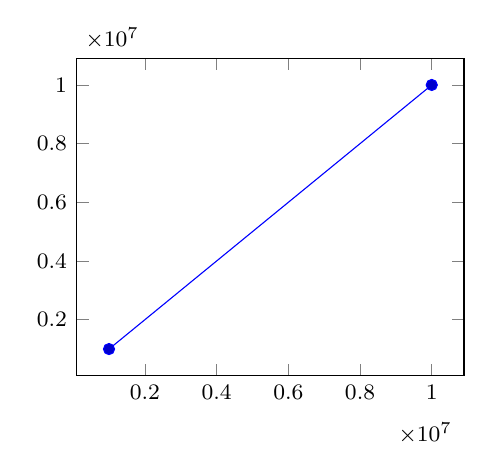
\begin{tikzpicture}
\begin{axis}[small,tick scale binop={\times}]
\addplot coordinates {(1e6,1e6) (1e7,1e7)};
\end{axis}
\end{tikzpicture}
\end{center}

\begin{latex}
% footnotesize = 
%  = 5cm x 4.31cm = 1.97in x 1.70in
\begin{tikzpicture}
\begin{axis}["footnotesize",tick scale binop={\times}]
\addplot coordinates {(1e6,1e6) (1e7,1e7)};
\end{axis}
\end{tikzpicture}
\end{latex}
%
\begin{center}
\tikzcount
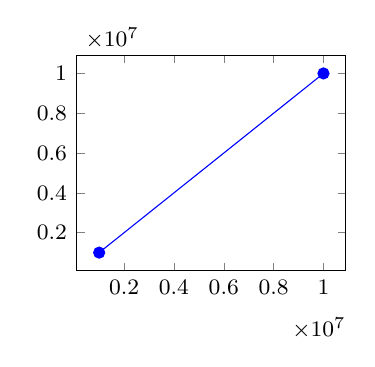
\begin{tikzpicture}
\begin{axis}[footnotesize,tick scale binop={\times}]
\addplot coordinates {(1e6,1e6) (1e7,1e7)};
\end{axis}
\end{tikzpicture}
\end{center}

\begin{latex}
% tiny = 
%  = 4cm x 3.45cm = 1.57in x 1.36in
\begin{tikzpicture}
\begin{axis}["tiny",tick scale binop={\times}]
\addplot coordinates {(1e6,1e6) (1e7,1e7)};
\end{axis}
\end{tikzpicture}
\end{latex}
% 
\begin{center}
\tikzcount
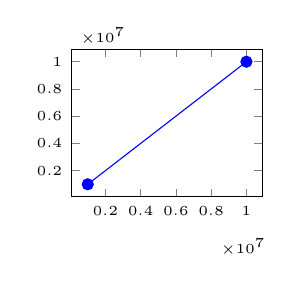
\begin{tikzpicture}
\begin{axis}[tiny,tick scale binop={\times}]
\addplot coordinates {(1e6,1e6) (1e7,1e7)};
\end{axis}
\end{tikzpicture}
\end{center}

Note that in each case the internal dimensions are the same, but the
external dimensions are getting smaller.  Note too that it's not just
the external dimensions that get smaller: various style settings are
adjusted so that the tick marks, and tick labels, all get smaller.
The result should be more legible and better appearance than if you
started with "normalsize" and then simply set "width" and "height"
directly to something like 4cm and 3.45cm.  

In each case, if you want to tweak the size, it's recommended you
first set it to the closest option out of "normalsize", "small",
"footnotesize" and "tiny" and then set "width" manually, and then
"pgfplots" will auto-scale "height" so that the aspect ratio is the
same as the normalsize, i.e.\ the aspect ratio equals $240/207 \approx
1.16$.  For instance, "small, width = 5.75cm".  You can set both
"width" and "height" in which case you get whatever aspect ratio you
have set.  Apparently the package has no direct provision for making
\emph{larger} plots.

\subsection{Setting external size manually}
So it remains to show you how to make things bigger than "normalsize"
and how to change the aspect ratio.  Here are three ways to make a
bigger plot, specifically one that is close to 25\% larger: (1) One we
manually set "width" and "height", (2) We scale the plot logically
(meaning all points get farther apart, but letters and lines don't
magnify), (3) we scale it visually (meaning it's like we put it under
a magnifying glass, making letters and numbers bigger and lines
thicker)


\begin{latex}
\begin{tikzpicture}
\begin{axis}["width=300pt, height=258.75pt", 
title = {Manually setting width and height}]
\addplot{x^2};
\end{axis}
\end{tikzpicture}
\end{latex}
%
\begin{center}
\tikzcount
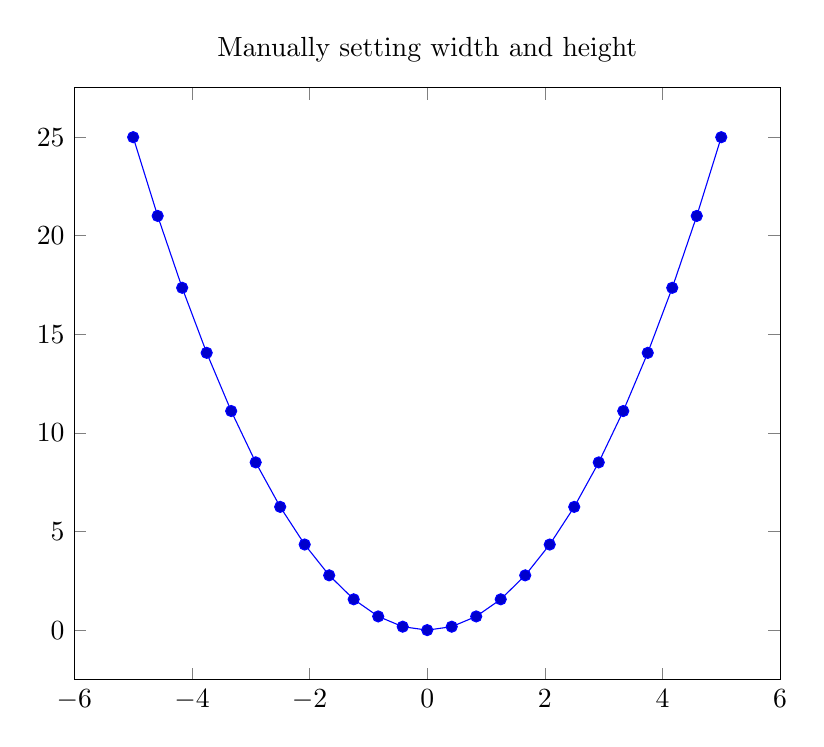
\begin{tikzpicture}
\begin{axis}[width=300pt, height=258.75pt, % width and height
title = {Manually setting width and height}]
\addplot{x^2};
\end{axis}
\end{tikzpicture}
\end{center}


\begin{latex}
\begin{tikzpicture}
\begin{axis}["scale=1.25,"
title = {Manually setting logical scale}] 
\addplot{x^2};
\end{axis}
\end{tikzpicture}
\end{latex}
%
\begin{center}
\tikzcount
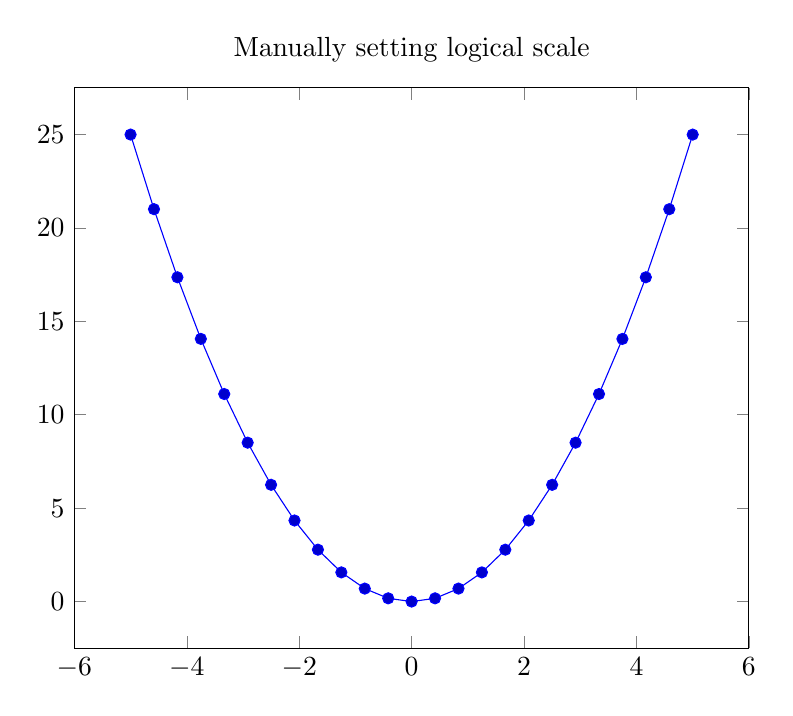
\begin{tikzpicture}
\begin{axis}[scale=1.25,
title = {Manually setting logical scale}] % logical scale
\addplot{x^2};
\end{axis}
\end{tikzpicture}
\end{center}


\begin{latex}
\begin{tikzpicture}["scale=1.25"] 
\begin{axis}[title = {Manually setting visual magnification}]
\addplot{x^2};
\end{axis}
\end{tikzpicture}
\end{latex}
% 
\begin{center}
\tikzcount
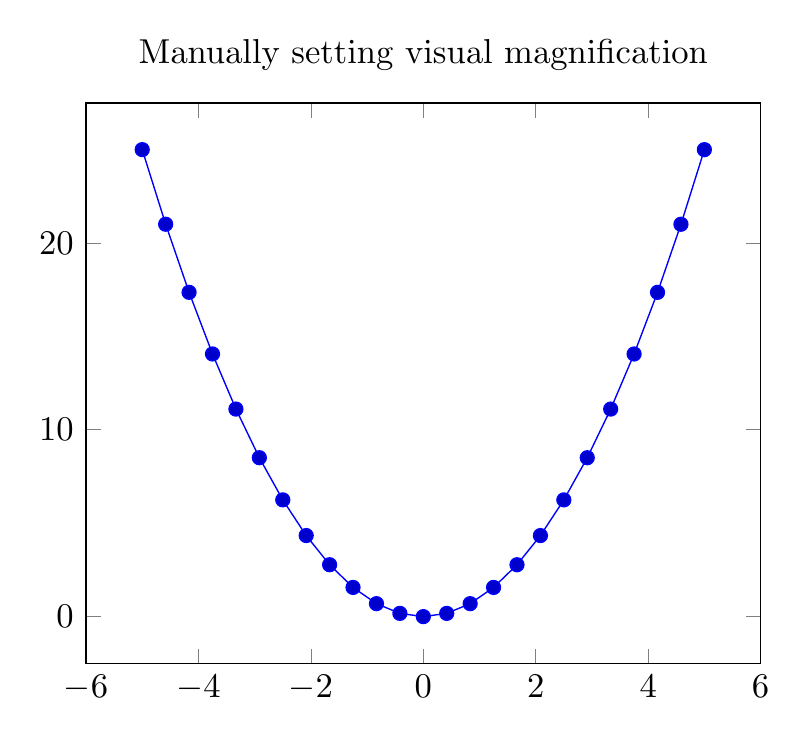
\begin{tikzpicture}[scale=1.25] % visual magnification
\begin{axis}[title = {Manually setting visual magnification}]
\addplot{x^2};
\end{axis}
\end{tikzpicture}
\end{center}
The first two are vaguely identical (probably the difference is how
the distances for tick marks, and tick labels are handled by "pgfplots").  The
disadvantage of the first one is that I had to both (1) guess what to
set the width, or remember that the original width is 240pt and then
increase that by 25\%, and (2) if I wanted to preserve the aspect
ratio then I had to calculate the height with a calculator (which is
what I did).

Note in the last one everything got larger, including the numbers and
the line thickness.  This could be an advantage if you are producing
something for a reader with a visual impairment.

Warning: it's pretty easy to forget (or not notice) the difference in
how to input the logical magnification and visual magnification: In
the former we put "scale=1.25" inside the "axis" options, and the
latter we put it inside the "tikzpicture" options.


\subsection{Setting external aspect ratio}
Sometimes you might want to override the default setting for the
external aspect ratio, like for the following graphs:
\begin{latex}
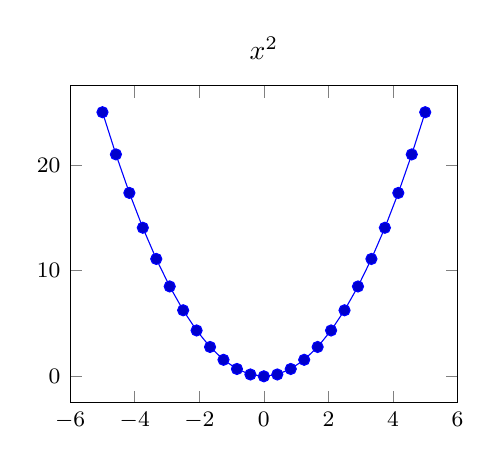
\begin{tikzpicture}
\begin{axis}[small,title={$x^2$}]
\addplot{x^2};
\end{axis}
\end{tikzpicture}%
~~%
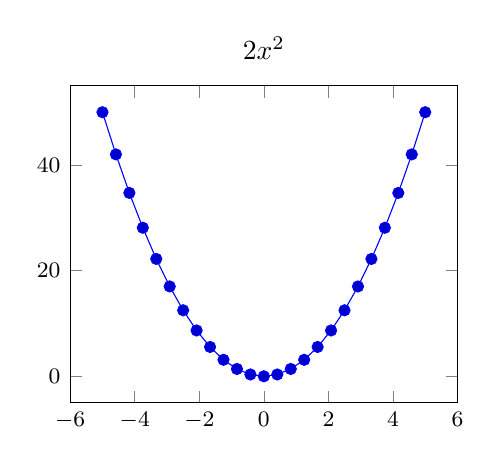
\begin{tikzpicture}
\begin{axis}[small,title={$2x^2$}]
\addplot{2*x^2};
\end{axis}
\end{tikzpicture}
\end{latex}
%
\begin{center}
\tikzcount
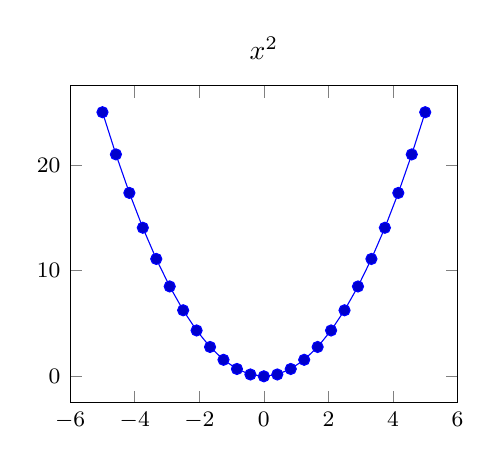
\begin{tikzpicture}
\begin{axis}[small,title={$x^2$}]
\addplot{x^2};
\end{axis}
\end{tikzpicture}%
~~%
\tikzcount
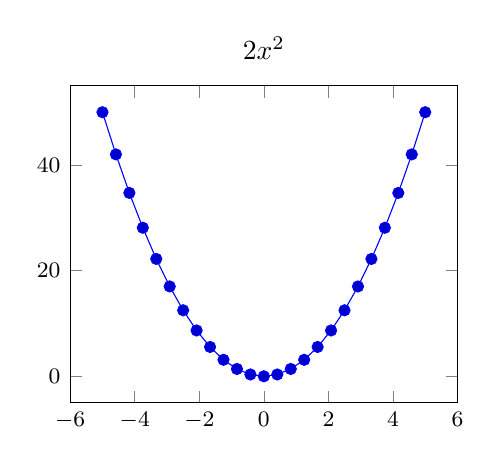
\begin{tikzpicture}
\begin{axis}[small,title={$2x^2$}]
\addplot{2*x^2};
\end{axis}
\end{tikzpicture}
\end{center}
If you were teaching students about vertical stretches, it sure might
be nice to have that second graph scaled to be twice as tall as the
first.  Here are two ways to get this done, the first probably being
the best
\begin{latex}
\begin{tikzpicture}
\begin{axis}[small,"y post scale=2"]
\addplot{2*x^2};
\end{axis}
\end{tikzpicture}%
~~%
\begin{tikzpicture}
\begin{axis}[small,"height=9cm"]
\addplot{2*x^2};
\end{axis}
\end{tikzpicture}
\end{latex}
%
\begin{center}
\tikzcount
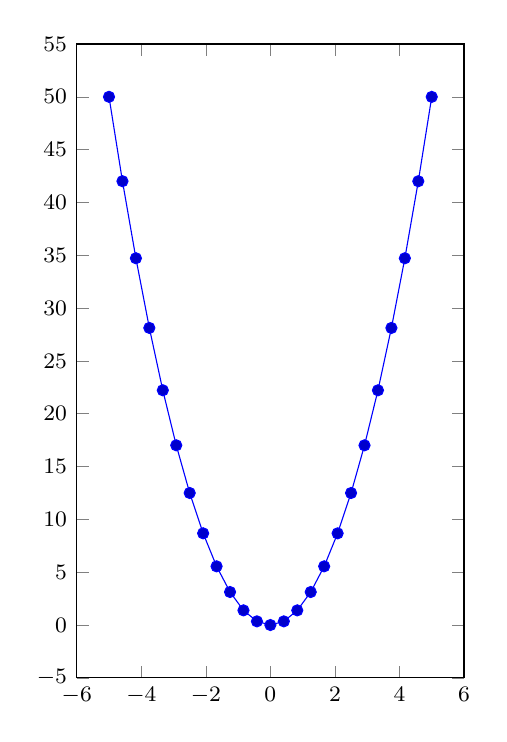
\begin{tikzpicture}
\begin{axis}[small,y post scale=2]
\addplot{2*x^2};
\end{axis}
\end{tikzpicture}%
~~%
\tikzcount
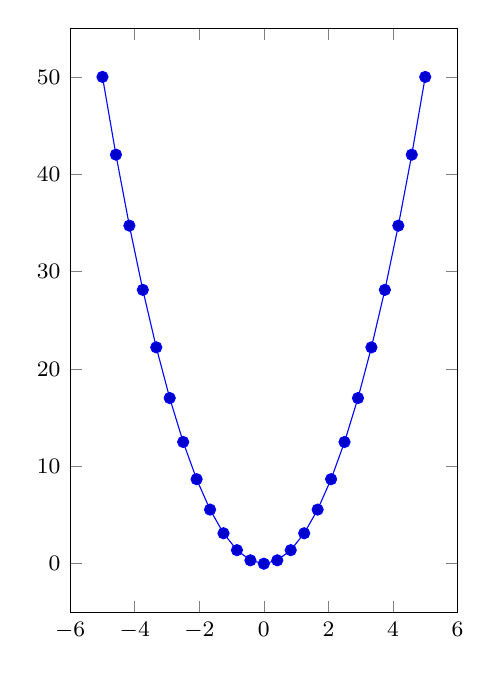
\begin{tikzpicture}
\begin{axis}[small,height=9cm]
\addplot{2*x^2};
\end{axis}
\end{tikzpicture}
\end{center}
The only small problem with the first way is remembering the key %
"y post scale" (I get this confused with the standard Tikz key
"yscale" which does \emph{not} work, see below).  The problem with the
second way is that I need to guess (or remember and calculate) the
number to set equal to height.


Here are two ways that do \emph{not} work.  The first because the
"unit vectors" and therefore the "unit vector ratio" for "axis" refers
to the \emph{internal axis} dimensions.
\begin{latex}
\begin{tikzpicture}
\begin{axis}[small,"unit vector ratio = 1 2"]
\addplot{2*x^2};
\end{axis}
\end{tikzpicture}%
~~%
\begin{tikzpicture}
\begin{axis}[small,"yscale=2"]
\addplot{2*x^2};
\end{axis}
\end{tikzpicture}
\end{latex}
%
\begin{center}
\tikzcount
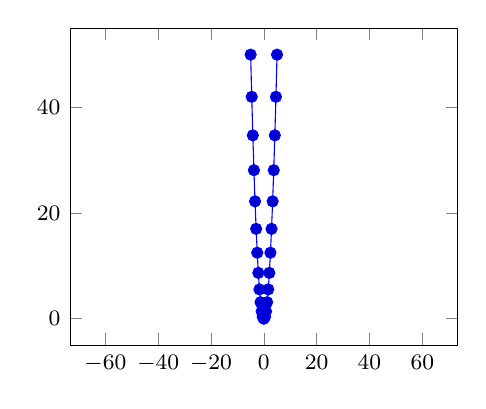
\begin{tikzpicture}
\begin{axis}[small,unit vector ratio = 1 2]
\addplot{2*x^2};
\end{axis}
\end{tikzpicture}%
~~%
\tikzcount
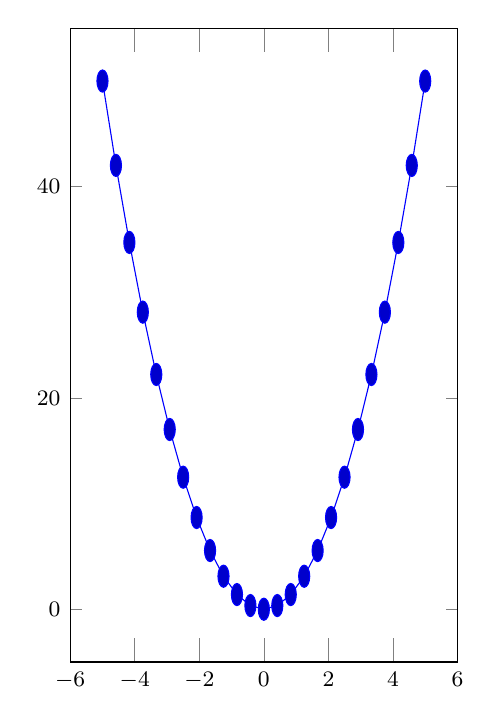
\begin{tikzpicture}
\begin{axis}[small,yscale=2]
\addplot{2*x^2};
\end{axis}
\end{tikzpicture}
\end{center}
% these work pretty OK, but are kind of complicated, or require
% obscure guesswork.
% \begin{tikzpicture}
% \begin{axis}[small,height=1.5*\pgfkeysvalueof{/pgfplots/width}]
% \addplot{2*x^2};
% \end{axis}
% \end{tikzpicture}%
% 
% \begin{tikzpicture}
% \begin{axis}[small,y=4] % the number here has to be guessed.
% \addplot{2*x^2};
% \end{axis}
% \end{tikzpicture}
Note that most of the scaling descriptions in the "pgfplots" manual
are for \emph{internal} lengths.  Thus "scale mode" and %
"unit vector ratio" and "axis equal" and "x=" and "y=", and similar
discussions about ``unit vectors'' and ``unit vector lengths'' are all
changes to the internal lengths. However, the "post scale" options
affect the external aspect ratio because they are applied after all
the other (internal) scaling has been done.

\subsection{Setting internal aspect ratio}
Note that there are certainly times where you might want to change the
internal aspect ratio (although clearly not in the above example with
$2x^2$).  For instance to make a circle look like a circle, or to
create a deliberate rescaling in internal units:
\begin{latex}
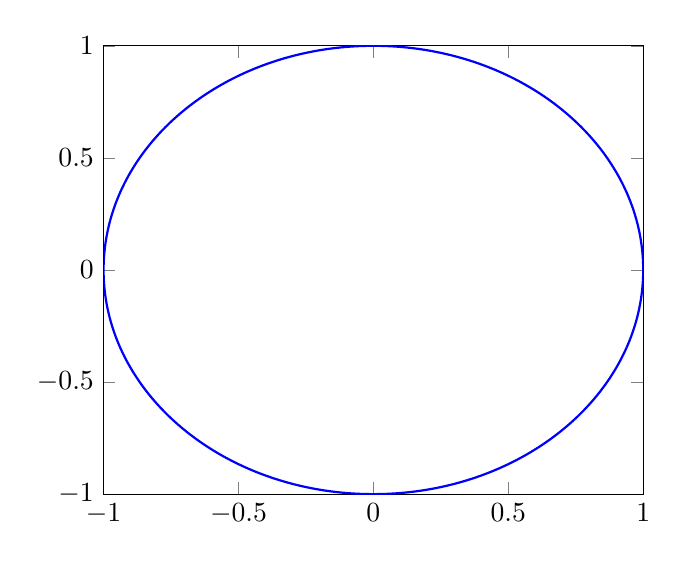
\begin{tikzpicture}
\begin{axis}[xmin = -1, xmax=1, ymin=-1,ymax=1]
\draw[thick,blue] (0,0) circle (1);
\end{axis}
\end{tikzpicture}%
~~%
\begin{tikzpicture}
\begin{axis}["axis equal",xmin = -1, xmax=1, ymin=-1,ymax=1]
\draw[thick,blue] (0,0) circle (1);
\end{axis}
\end{tikzpicture}
\end{latex}

\tikzcount
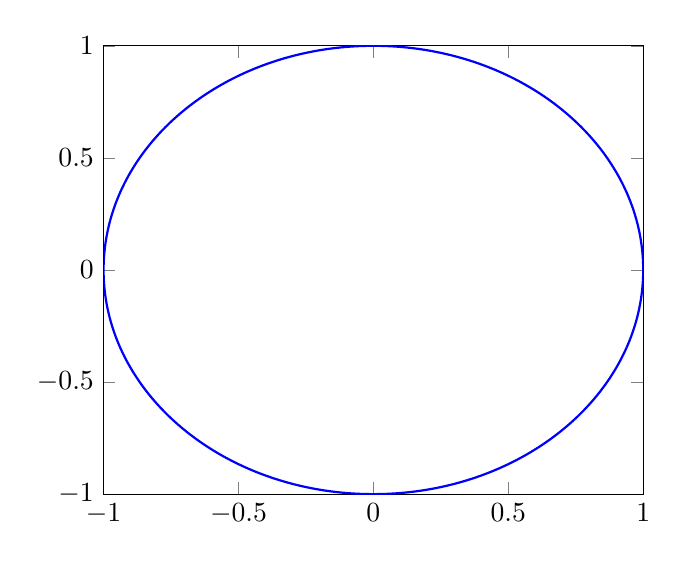
\begin{tikzpicture}
\begin{axis}[xmin = -1, xmax=1, ymin=-1,ymax=1]
\draw[thick,blue] (0,0) circle (1);
\end{axis}
\end{tikzpicture}
~~
\tikzcount
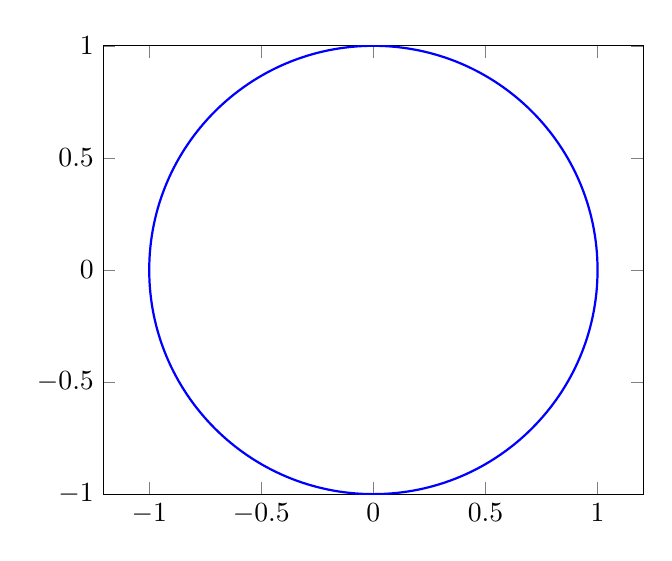
\begin{tikzpicture}
\begin{axis}[axis equal,xmin = -1, xmax=1, ymin=-1,ymax=1]
\draw[thick,blue] (0,0) circle (1);
\end{axis}
\end{tikzpicture}
Note that the keys "axis equal" and settings for "xmin", "xmax" are
somewhat contradictory (given the fact that "pgfplots" is not going to
automatically change the \emph{external} dimensions of this picture),
so "pgfplots" tries the best it can, but in the end "axis equal" wins
and you can see the picture extends beyond the "xmin" and "xmax"
settings.

Here's an example where we purposely do want to make one graph
skinnier: 
\begin{latex}
\begin{center}
Note that $10(x-10)^2$ is ``skinnier'' than $x^2$\\
\begin{tikzpicture}
\begin{axis}["unit vector ratio = 20 1",
     axis lines=middle]
\addplot[smooth,thick,blue, domain=0:20]
  {10*(x-10)^2} node[pos=0.8,below right]{$y=10(x-10)^2$};
\end{axis}
\end{tikzpicture}%
~~%
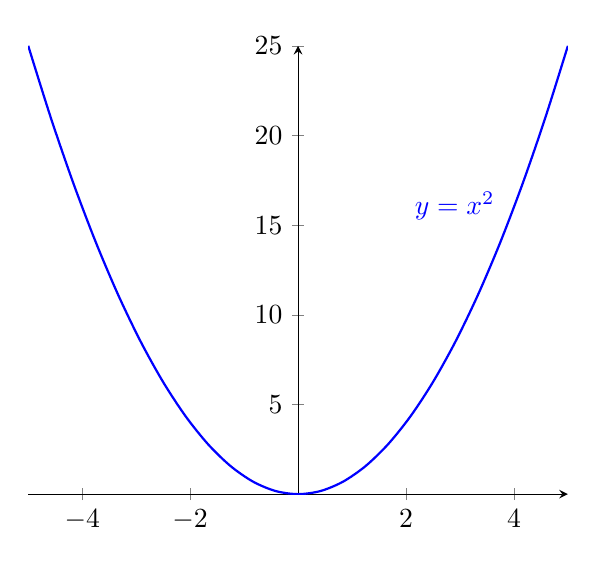
\begin{tikzpicture}
\begin{axis}[ axis lines=middle]
\addplot[smooth,thick,blue]  {x^2} node[pos=0.8, above left]{$y=x^2$};
\end{axis}
\end{tikzpicture}
\end{center}
\end{latex}
%
\begin{center}
Note that $10(x-10)^2$ is ``skinnier'' than $x^2$\\
\tikzcount
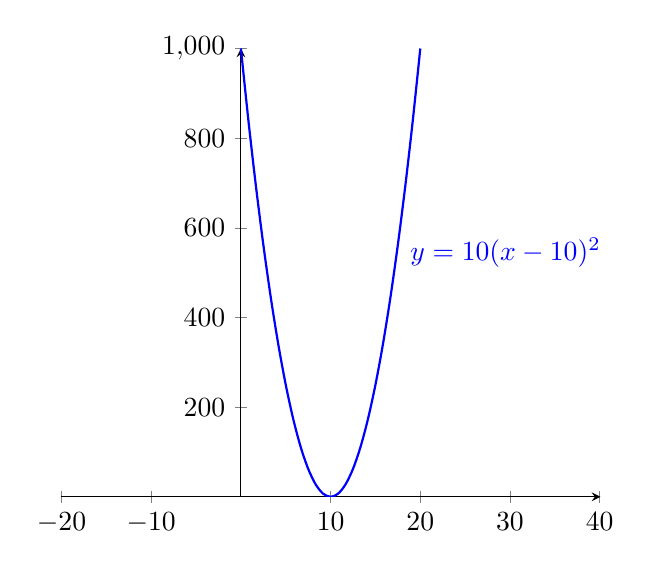
\begin{tikzpicture}
\begin{axis}[unit vector ratio = 20 1,
     axis lines=middle]
\addplot[smooth,thick,blue, domain=0:20]
  {10*(x-10)^2} node[pos=0.8,below right]{$y=10(x-10)^2$};
\end{axis}
\end{tikzpicture}
~~
\tikzcount
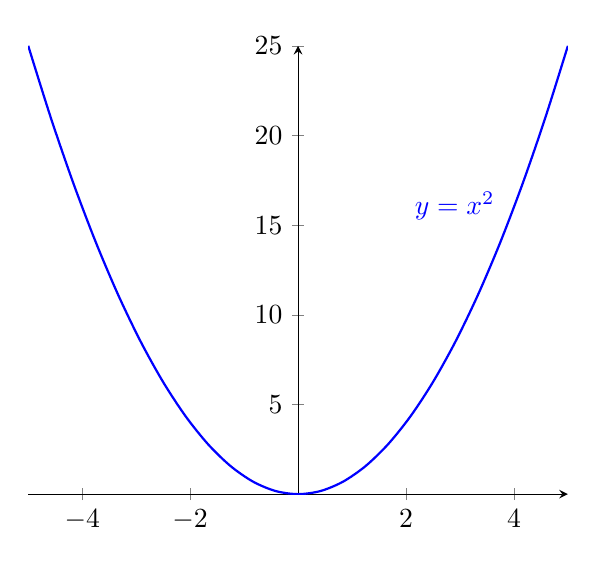
\begin{tikzpicture}
\begin{axis}[ axis lines=middle]
\addplot[smooth,thick,blue]  {x^2} node[pos=0.8, above left]{$y=x^2$};
\end{axis}
\end{tikzpicture}
\end{center}
Here we manually set the internal aspect ratio because otherwise
"pgfplots" does too good of a job auto-scaling these pictures and they
end up looking the same!  (Also, we did not scale the external
picture, unlike an earlier example because, for whatever reason, we
wanted the figures to be the same size.) 



%%% Local Variables:
%%% mode: latex
%%% TeX-master: "../pgfplots_tutorial"
%%% End:
